\section{Introduction}
\label{sec:intro}

Spatiotemporal reasoning requires models to combine heterogeneous forms of computation, including geometric localization, temporal relation reasoning, route planning, trajectory analysis, and graph-structured inference~\citep{quan2025benchmarking,li2025stbench,ni2026streasoner}.
Complex queries often invoke these computations sequentially, where downstream steps depend strictly on intermediate results produced by earlier ones. Consequently, the core challenge lies not just in executing individual computations, but in determining \textit{which} specialist should act next as the execution unfolds. We study this under the lens of \emph{failure-aware specialist routing}: determining the optimal next specialist given the current agent, the task type, and, crucially, the observed execution outcome.

This question is especially important when execution deviates from the nominal path.
Failures in specialist pipelines are not monolithic: an agent may produce a malformed output, become blocked because a required upstream result is missing, or fail because its tool menu cannot resolve the query.
These cases require different routing decisions, such as retrying with a sibling specialist, rerouting to an upstream producer, or escalating to another agent family.
However, existing tool-augmented and multi-agent LLM systems often leave such control decisions implicit in language generation, making recovery difficult to inspect, optimize, and reuse across executions~\citep{wei2026beyond,li2024survey}.

\begin{figure}[!htbp]
\centering
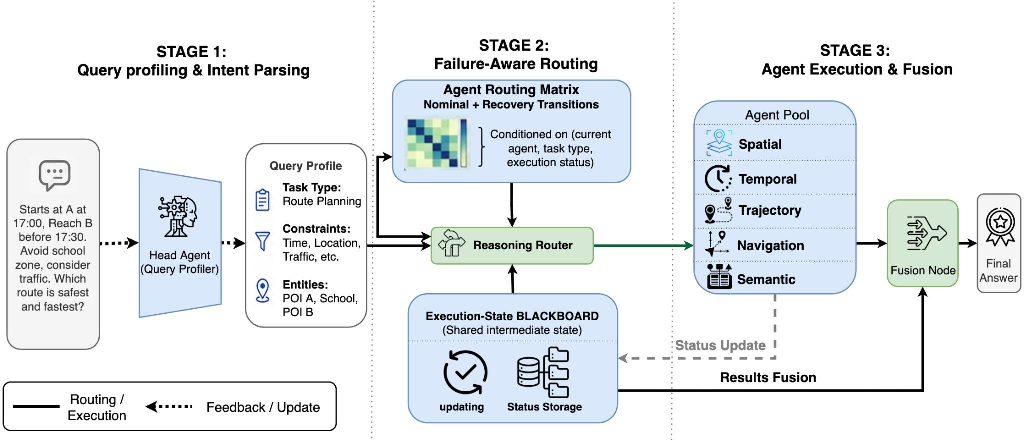
\includegraphics[width=0.95\textwidth]{figures/star_figure_1.pdf}
\caption{\starname{} architecture. Queries are parsed into a task profile, the failure-aware routing matrix selects specialists conditioned on the current agent, task type, execution status, and specialists execute through an extract-compute-deposit protocol over a shared blackboard before final fusion.}
\label{fig:framework}
\end{figure}

This paper proposes \starname{} (\textbf{S}patio-\textbf{T}emporal \textbf{A}gent \textbf{R}outer), a failure-aware routing framework that externalizes inter-agent control into a state-conditioned transition policy.
At the center of \starname{} is an agent routing matrix indexed by the current agent, task type, execution status, and next agent.
The matrix combines expert-specified nominal routes for successful execution with recovery transitions learned from execution traces.
By conditioning on typed statuses such as malformed output, missing dependency, and tool--query mismatch, \starname{} treats recovery as an explicit routing problem rather than as an implicit byproduct of LLM generation. Specialists execute through a tool-grounded \emph{extract--compute--deposit} protocol.
The LLM selects a computation and extracts its parameters, deterministic tools perform the computation, and the resulting intermediate state is deposited into a shared blackboard for downstream agents and final fusion.
This protocol exposes typed execution outcomes to the router and provides the intermediate state needed for recovery transitions.

Our central claim is that typed execution feedback should be treated as a first-class control signal for multi-agent reasoning.
Structurally, retaining unsuccessful traces enlarges the support of the learned routing policy on error states, enabling recovery transitions that success-only training cannot represent.
Throughout experiments, \starname{} improves over LLM-only, prompting-based, and agentic baselines.
Router-specific ablations and recovery analyses further show that the gains are concentrated on executions that deviate from the nominal route, isolating the contribution of failure-aware routing rather than specialist composition alone. Our key \textbf{contributions} are:

\begin{enumerate}[leftmargin=*,itemsep=1pt]
    \item \textbf{Failure-aware specialist routing.}
     \starname{} formulates specialist composition as a state-conditioned routing problem over the current agent, task type, and typed execution status, making recovery decisions explicit rather than leaving them implicit in language generation.

    \item \textbf{An interpretable agent routing matrix.}
    A routing matrix is introduced combining expert nominal routes with learned recovery transitions from execution traces.
    The matrix conditions on distinct failure modes, including malformed outputs, missing dependencies, and tool--query mismatches.

    \item \textbf{Tool-grounded execution with shared intermediate state.}
    The routing policy is instantiated in a spatiotemporal multi-agent system where specialists follow an extract--compute--deposit protocol and write intermediate results to a shared blackboard for downstream fusion.

    \item \textbf{Structural and empirical evidence for recovery-aware routing.}
    Experiment results proved that retaining unsuccessful traces enables recovery transitions that success-only training cannot represent.
    Across three benchmarks and eight backbone LLMs, router-specific ablations and recovery analyses demonstrate that typed failure-aware routing improves robustness especially on executions that deviate from the nominal path.
\end{enumerate}